\chapter{RE-008 --- Byte-Packed Surface Representation}\label{record-250}

\noindent{\footnotesize\color{BookMuted}\path{docs/design/0001-008-byte-packed-surface-representation/008-byte-packed-surface-representation.md}\par}\smallskip

Source backlog item: \texttt{d\allowbreak{}o\allowbreak{}c\allowbreak{}s\allowbreak{}/\allowbreak{}m\allowbreak{}e\allowbreak{}t\allowbreak{}h\allowbreak{}o\allowbreak{}d\allowbreak{}/\allowbreak{}b\allowbreak{}a\allowbreak{}c\allowbreak{}k\allowbreak{}l\allowbreak{}o\allowbreak{}g\allowbreak{}/\allowbreak{}a\allowbreak{}s\allowbreak{}a\allowbreak{}p\allowbreak{}/\allowbreak{}R\allowbreak{}E\allowbreak{}\_\allowbreak{}0\allowbreak{}0\allowbreak{}8\allowbreak{}-\allowbreak{}b\allowbreak{}y\allowbreak{}t\allowbreak{}e\allowbreak{}-\allowbreak{}p\allowbreak{}a\allowbreak{}c\allowbreak{}k\allowbreak{}e\allowbreak{}d\allowbreak{}-\allowbreak{}s\allowbreak{}u\allowbreak{}r\allowbreak{}f\allowbreak{}a\allowbreak{}c\allowbreak{}e\allowbreak{}-\allowbreak{}r\allowbreak{}e\allowbreak{}p\allowbreak{}r\allowbreak{}e\allowbreak{}s\allowbreak{}e\allowbreak{}n\allowbreak{}t\allowbreak{}a\allowbreak{}t\allowbreak{}i\allowbreak{}o\allowbreak{}n\allowbreak{}.\allowbreak{}m\allowbreak{}d} Legend: RE

\section{Sponsors}\label{record-250-sponsors}

\begin{itemize}
\tightlist
\item
  Human: James
\item
  Agent: Claude (Opus 4.6)
\end{itemize}

\section{Hill}\label{record-250-hill}

Surface rendering in Bijou goes from ``every cell is a heap-allocated object with string colors'' to ``every cell is 10 bytes in a flat typed array with numeric RGB.'' The DOGFOOD landing benchmark is at parity or faster than the pre-RE-008 baseline, and the architecture enables zero-allocation rendering for any component that opts into \texttt{s\allowbreak{}e\allowbreak{}t\allowbreak{}R\allowbreak{}G\allowbreak{}B\allowbreak{}(\allowbreak{})}.

\section{Playback Questions}\label{record-250-playback-questions}

\subsection{Human}\label{record-250-human}

\begin{itemize}
\tightlist
\item[$\boxtimes$]
  Does the DOGFOOD landing render at least as fast as before?
\item[$\boxtimes$]
  Are all 2816 existing tests still passing?
\item[$\boxtimes$]
  Is the \texttt{s\allowbreak{}e\allowbreak{}t\allowbreak{}(\allowbreak{})} convenience API preserved and documented?
\item[$\boxtimes$]
  Can components opt into the fast path incrementally?
\end{itemize}

\subsection{Agent}\label{record-250-agent}

\begin{itemize}
\tightlist
\item[$\boxtimes$]
  Is the packed buffer the source of truth, with Cell{[}{]} as lazy decode?
\item[$\boxtimes$]
  Does the differ operate on bytes, not strings?
\item[$\boxtimes$]
  Does blit copy bytes directly between packed buffers?
\item[$\boxtimes$]
  Are side-table chars (emoji, grapheme clusters) handled correctly?
\end{itemize}

\section{What Shipped}\label{record-250-what-shipped}

\subsection{Architecture}\label{record-250-architecture}

\begin{itemize}
\tightlist
\item
  \textbf{Packed cell encoding} (\texttt{p\allowbreak{}a\allowbreak{}c\allowbreak{}k\allowbreak{}e\allowbreak{}d\allowbreak{}-\allowbreak{}c\allowbreak{}e\allowbreak{}l\allowbreak{}l\allowbreak{}.\allowbreak{}t\allowbreak{}s}): 10-byte layout per cell --- uint16 char, 3B fg RGB, 3B bg RGB, 1B flags bitfield, 1B alpha/presence. Side table for multi-codepoint graphemes outside the BMP.
\item
  \textbf{Lazy dirty bitmap}: \texttt{U\allowbreak{}i\allowbreak{}n\allowbreak{}t\allowbreak{}3\allowbreak{}2\allowbreak{}A\allowbreak{}r\allowbreak{}r\allowbreak{}a\allowbreak{}y} bitmap (1 bit per cell) tracks which cells need decoding from the buffer. Writes mark dirty; reads decode on demand.
\item
  \textbf{\texttt{s\allowbreak{}e\allowbreak{}t\allowbreak{}R\allowbreak{}G\allowbreak{}B\allowbreak{}(\allowbreak{})} API}: Zero-allocation writes --- char code + numeric RGB directly into the buffer. No hex parsing, no Cell object.
\item
  \textbf{Packed blit}: 10-byte memcpy per cell with side-table re-encoding for cross-surface grapheme clusters.
\item
  \textbf{Template-stamp fill/clear}: Encode once, copy bytes to every position.
\item
  \textbf{Direct ANSI emission}: Differ reads RGB bytes from the buffer and emits \texttt{\textbackslash{}\allowbreak{}x\allowbreak{}1\allowbreak{}b\allowbreak{}[\allowbreak{}3\allowbreak{}8\allowbreak{};\allowbreak{}2\allowbreak{};\allowbreak{}R\allowbreak{};\allowbreak{}G\allowbreak{};\allowbreak{}B\allowbreak{}m} directly, with a style-byte hash cache. Bypasses chalk and StylePort entirely on the hot diff path.
\item
  \textbf{Numeric theme tokens}: \texttt{T\allowbreak{}o\allowbreak{}k\allowbreak{}e\allowbreak{}n\allowbreak{}V\allowbreak{}a\allowbreak{}l\allowbreak{}u\allowbreak{}e\allowbreak{}.\allowbreak{}f\allowbreak{}g\allowbreak{}R\allowbreak{}G\allowbreak{}B} / \texttt{b\allowbreak{}g\allowbreak{}R\allowbreak{}G\allowbreak{}B} pre-parsed at theme resolution time.
\end{itemize}

\subsection{Slices (19 commits)}\label{record-250-slices-19-commits}

\begin{enumerate}
\def\labelenumi{\arabic{enumi}.}
\tightlist
\item
  Packed-cell byte encoding module
\item
  \texttt{c\allowbreak{}r\allowbreak{}e\allowbreak{}a\allowbreak{}t\allowbreak{}e\allowbreak{}S\allowbreak{}u\allowbreak{}r\allowbreak{}f\allowbreak{}a\allowbreak{}c\allowbreak{}e} backed by \texttt{U\allowbreak{}i\allowbreak{}n\allowbreak{}t\allowbreak{}8\allowbreak{}A\allowbreak{}r\allowbreak{}r\allowbreak{}a\allowbreak{}y} + eager sync
\item
  Route all direct cell mutations through \texttt{s\allowbreak{}u\allowbreak{}r\allowbreak{}f\allowbreak{}a\allowbreak{}c\allowbreak{}e\allowbreak{}.\allowbreak{}s\allowbreak{}e\allowbreak{}t\allowbreak{}(\allowbreak{})}
\item
  Packed byte-comparison differ
\item
  Grayscale middleware on packed bytes
\item
  Lazy dirty bitmap (replace eager sync)
\item
  Zero-alloc hex parsing (charCode arithmetic, lookup table)
\item
  Inline hex→RGB, FULL\_MASK fast path, numeric theme tokens
\item
  Direct ANSI SGR emission with cached style-byte hash
\item
  \texttt{s\allowbreak{}e\allowbreak{}t\allowbreak{}R\allowbreak{}G\allowbreak{}B\allowbreak{}(\allowbreak{})} API + perf-gradient demo migration
\item
  Packed byte-copy blit
\item
  Template-stamp fill, clear, clone
\item
  Component migration: surface-text, box-v3, separator-v3
\item
  Component migration: overlay dim, flex/overlay bg inheritance
\item
  Component migration: table-v3, alert-v3
\item
  Component migration: notification, css/text-style
\item
  Component migration: badge, focus-area, preference-list, canvas, differ
\end{enumerate}

\subsection{Benchmark Results}\label{record-250-benchmark-results}

\begin{center}
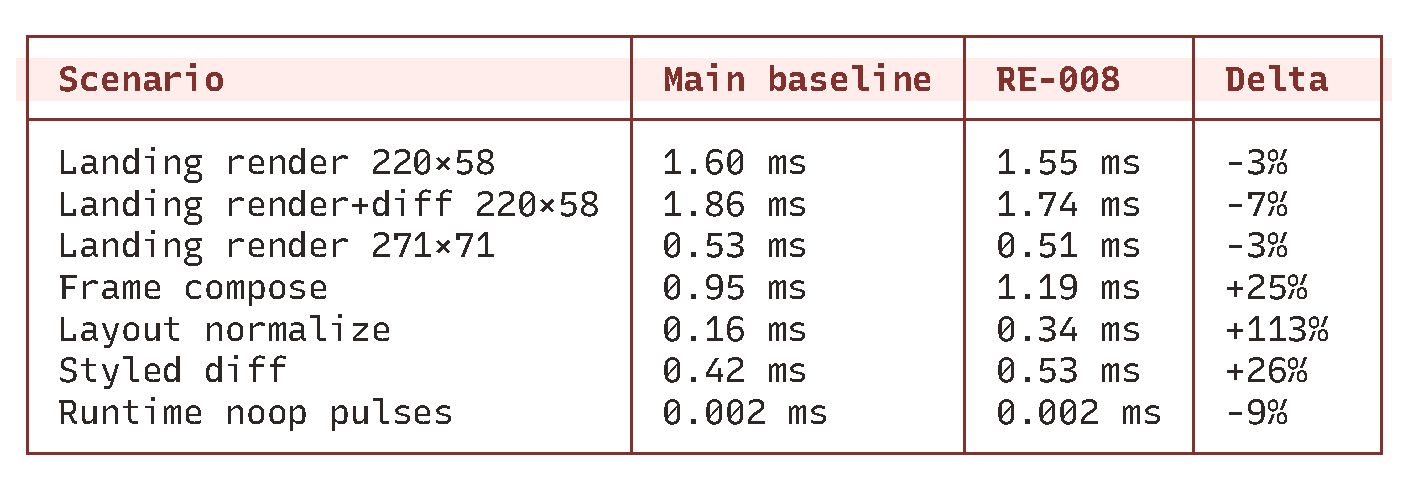
\includegraphics[width=\linewidth]{figures/tables/table-064-g1-1.pdf}
\par\smallskip{\scriptsize\color{BookMuted}Rows 1–7. Actual Bijou table component.}
\end{center}


Real-world DOGFOOD rendering is faster. Synthetic stress tests still show overhead from the \texttt{s\allowbreak{}e\allowbreak{}t\allowbreak{}(\allowbreak{})} hex-parsing path --- these will improve as more rendering paths move to direct byte manipulation.

\section{Accessibility and Assistive Reading}\label{record-250-accessibility-and-assistive-reading}

No user-facing changes. The packed buffer is internal; all public APIs return the same Cell objects and string output as before.

\section{Localization and Directionality}\label{record-250-localization-and-directionality}

No changes. Character encoding handles the full Unicode BMP directly and uses a side table for astral/multi-codepoint graphemes.

\section{Agent Inspectability and Explainability}\label{record-250-agent-inspectability-and-explainability}

The \texttt{P\allowbreak{}a\allowbreak{}c\allowbreak{}k\allowbreak{}e\allowbreak{}d\allowbreak{}S\allowbreak{}u\allowbreak{}r\allowbreak{}f\allowbreak{}a\allowbreak{}c\allowbreak{}e} interface and \texttt{s\allowbreak{}e\allowbreak{}t\allowbreak{}R\allowbreak{}G\allowbreak{}B\allowbreak{}(\allowbreak{})} API are exported and documented. Agents can query surface dimensions, read cells via \texttt{g\allowbreak{}e\allowbreak{}t\allowbreak{}(\allowbreak{})}, and use the packed buffer for performance-sensitive rendering.

\section{Non-goals}\label{record-250-non-goals}

\begin{itemize}
\tightlist
\item
  Changing the public Cell interface or breaking component APIs
\item
  Removing hex color support from the convenience \texttt{s\allowbreak{}e\allowbreak{}t\allowbreak{}(\allowbreak{})} API
\item
  Pre-allocated output buffer for stdout (deferred to future work)
\item
  Eliminating the Cell{[}{]} layer entirely (the lazy decode + dirty bitmap keeps backward compatibility with minimal overhead)
\end{itemize}

